This example on the Van der Pol oscillator shows how to use BFilt for non-linear continuous-discrete model. Here the van\_\-der\_\-pol class : \begin{Desc}
\item[]van\_\-der\_\-pol.h 

\begin{DocInclude}\begin{verbatim}#ifndef __VAN_DER_POL
#define __VAN_DER_POL


#include <bfilt/gaussian_model.h>


class Van_Der_Pol : public Continuous_Discrete_Model
{
public :
      double lambda;
      
      Van_Der_Pol(void);
      dcovector Drift_Function(const dcovector & X);
      dgematrix J_Drift_Function(const dcovector & X);
      dcovector Observation_Function(const dcovector& X);
      dgematrix J_Observation_Function(const dcovector & X);
      dgematrix Diffusion_Function(void);
};


#endif
\end{verbatim}
\end{DocInclude}
 van\_\-der\_\-pol.cpp 

\begin{DocInclude}\begin{verbatim}#include "van_der_pol.h"

Van_Der_Pol::Van_Der_Pol(void)
{
      lambda = 3.;

      Qw.resize(1);
      Qw(0,0)= 1.;
      Qv.resize(1);
      Qv(0,0)=0.1;
  
      X0.resize(2);
      X0(0) = 0.5;
      X0(1) = 0.5;
      R0.resize(2);
      R0.zero();
      R0(0,0)=0.;
      R0(1,1)=.1;
      Ts=.1;

}


dcovector Van_Der_Pol::Drift_Function(const dcovector & X)
{
      dcovector dX(X.l);

      dX(0) = X(1);
      dX(1) = lambda * (1. - X(0) * X(0)) * X(1) - X(0);

      return dX;
}

dgematrix Van_Der_Pol::J_Drift_Function(const dcovector & X)
{
      dgematrix F(X.l,X.l);

      F(0,0) = 0.;
      F(0,1) = 1.;
      F(1,0) = -2. * lambda * X(0) * X(1);
      F(1,1) = - lambda * X(0) * X(0);

      return F;
}
dcovector Van_Der_Pol::Observation_Function(const dcovector& X)
{
      dcovector Y(1);
      Y(0) = X(0);
      return Y;
}

dgematrix Van_Der_Pol::J_Observation_Function(const dcovector & X)
{
      dgematrix H(1,2);
      H(0,0) = 0.;
      H(0,1) = 1.;
      return H;
}
dgematrix Van_Der_Pol::Diffusion_Function(void)
{
      dgematrix G(2,1);
      G(0,0) = 0.;
      G(1,0) = 1.;

      return G;
}
\end{verbatim}
\end{DocInclude}
 The main program : 

\begin{DocInclude}\begin{verbatim}#include <bfilt/simulator.h>
#include <bfilt/extended_kalman_filter.h>
#include "van_der_pol.h"



int main(int argc, char **argv)
{
      Van_Der_Pol model;              // The model

      CD_Simulator sim(&model);   // The simulator
      
      CD_Extended_Kalman_Filter  filter(&model,THGL);      // The filter
      
      // Simulation 40 seconds
      sim.Simulate(40.);
        

      // Filtering from the simulated output sim.Y
      filter.Filtering(sim.Y);

      // Output Files for simulation
      sim.Save_Y("output.dat");
      sim.Save_X("state.dat");

      // Output File for filtering
      filter.Save_X("estimation.dat");
 
      return 0;
}
\end{verbatim}
\end{DocInclude}
 Results can be plotted (here with gnuplot):  \begin{ImageNoCaption}\mbox{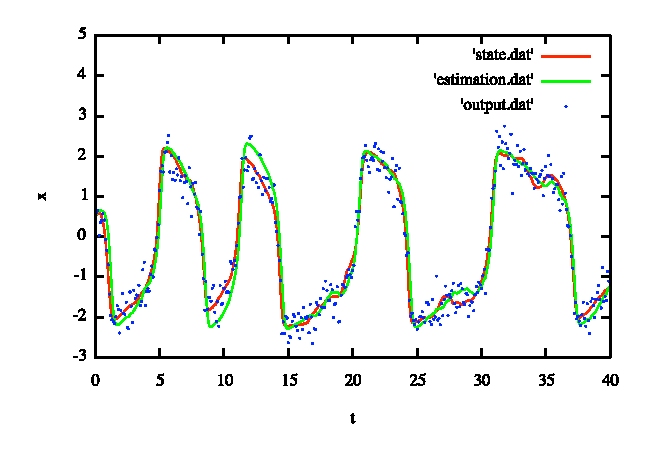
\includegraphics{van_der_pol}}
\end{ImageNoCaption}
 \end{Desc}
